\documentclass[10pt]{beamer}

\usetheme[progressbar=frametitle]{metropolis}
\usepackage{appendixnumberbeamer}
\usepackage{lipsum}
\usepackage{amsmath}
\usepackage{amssymb}
\usepackage{mathtools}
\usepackage{booktabs}
\usepackage{hyperref}
\usepackage[scale=2]{ccicons}
\usepackage{pgfplots}
\usepgfplotslibrary{dateplot}
\usepackage{dirtytalk}
\usepackage{xspace}
\usepackage{fancybox}
\usepackage{enumerate}
\usepackage[ruled,vlined]{algorithm2e}
\usepackage{algorithmic}
\usepackage{tikz}
\allowdisplaybreaks
\newcommand{\themename}{\textbf{\textsc{metropolis}}\xspace}
\newcommand*\circled[1]{\tikz[baseline=(char.base)]{
            \node[shape=circle,draw,inner sep=2pt] (char) {#1};}}

\DeclarePairedDelimiter\ceil{\lceil}{\rceil}
\DeclarePairedDelimiter\floor{\lfloor}{\rfloor}
\newcommand{\Cross}{\mathbin{\tikz [x=1.1ex,y=1.1ex,line width=.1ex] \draw (0,0) -- (1,1) (0,1) -- (1,0);}}%
\hypersetup{
    colorlinks=true,
    linkcolor=blue,
    filecolor=magenta,      
    urlcolor=cyan,
}
\definecolor{mpigreen}{HTML}{005f79}
\setbeamercolor{frametitle}{bg=mpigreen}

\title{Branch \& Bound per TSP simmetrico}

\author{Lorenzo Sciandra, \and Stefano Vittorio Porta}
\date{A.A. 2020-2021}
\institute{Università degli Studi di Torino}
\titlegraphic{\hfill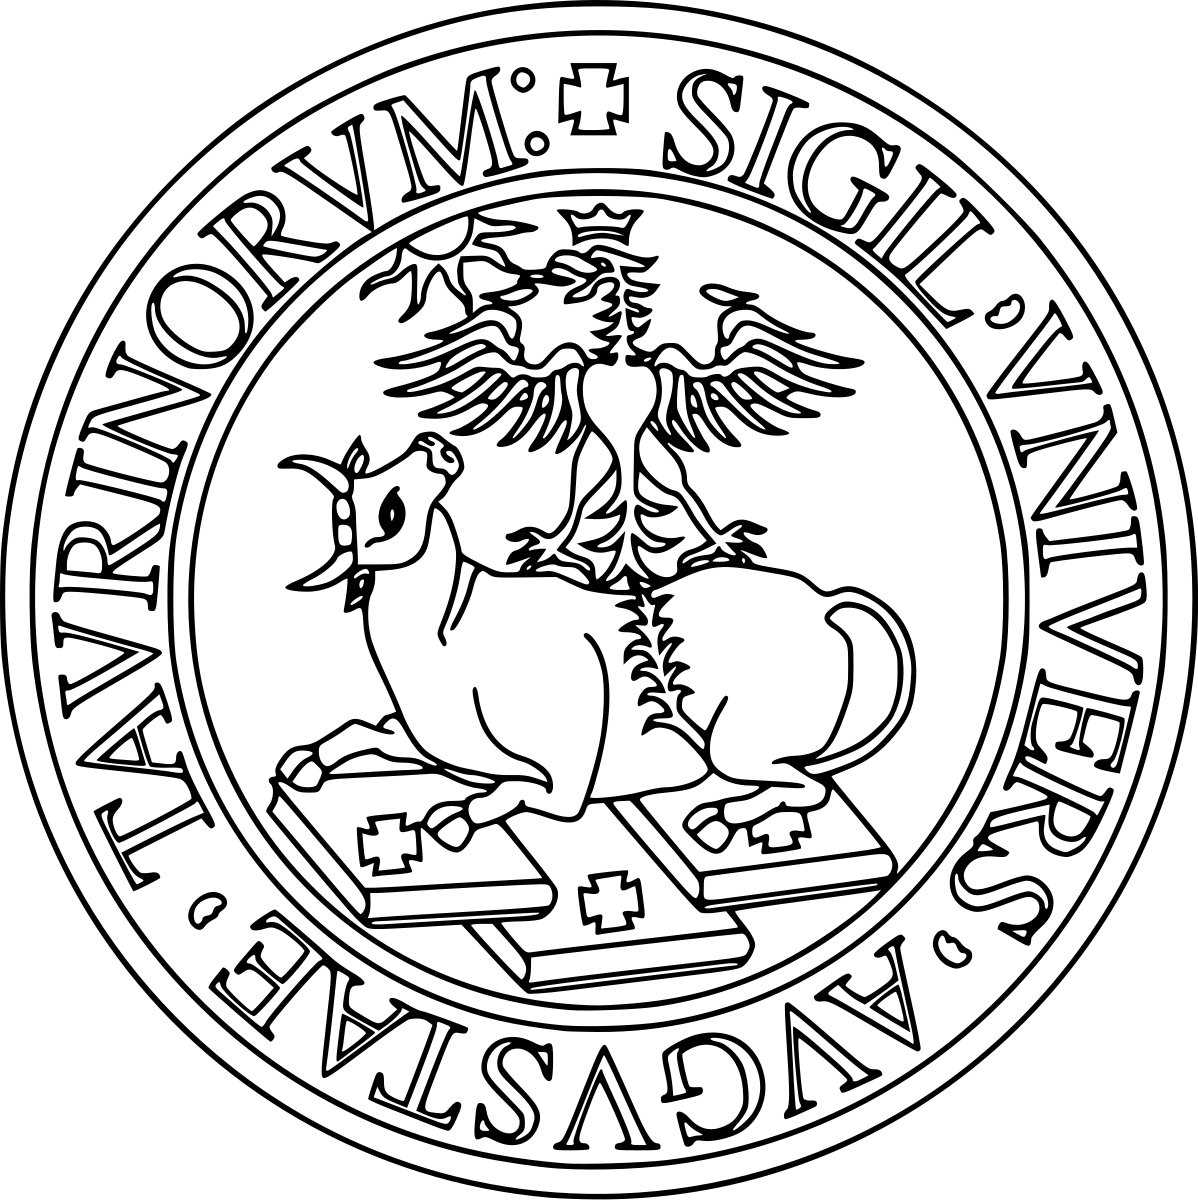
\includegraphics[height=2cm]{files/Unito-logo.png}}

\hypersetup{colorlinks,linkcolor=,urlcolor=red}
\setbeamertemplate{section in toc}{\inserttocsectionnumber.~\inserttocsection}

\begin{document}


\maketitle

\section{Indice argomenti}

\begin{frame}{Indice argomenti}
    \tableofcontents
\end{frame}

\section{Introduzione al TSP simmetrico}
\begin{frame}{TSP simmetrico}
    Il problema del commesso viaggiatore, spesso indicato come \textbf{Travelling Salesman Problem} nella sua più tipica rappresentazione chiede:\newline
    "\textit{Dato un insieme di città, e note le distanze tra ciascuna coppia di esse, trovare il tragitto di minima percorrenza che un commesso viaggiatore deve seguire per visitare tutte le città una ed una sola volta e ritornare alla città di partenza.}"
    \newline
    \newline
    Il TSP è un problema NP-hard, nella precisione NP-completo e quindi gli algoritmi che lo risolvono all'ottimo richiedono una complessità in tempo più che polinomiale nell'istanza trattata ($P \neq NP)$.
\end{frame}

\begin{frame}{TSP simmetrico}
    Per modellare il TSP simmetrico si usa un grafo non orientato $G=(V,E)$ con costi $c_{ij}$ associati agli archi, da cui si richiede di determinare un insieme di archi $C^* \subset E$ con costo minimo possibile. Tale insieme $C^*$ deve formare un \textit{circuito hamiltoniano}, cioè un circuito che passi una ed una sola volta per ogni nodo del grafo. Il problema che analizzeremo è la versione simmetrica del TSP ossia $c_{ij} = c_{ji} \:\: \forall i,j \in V$. Ogni arco è quindi percorribile in entrambe le direzioni spendendo lo stesso costo.
    \begin{figure}
        \centering
        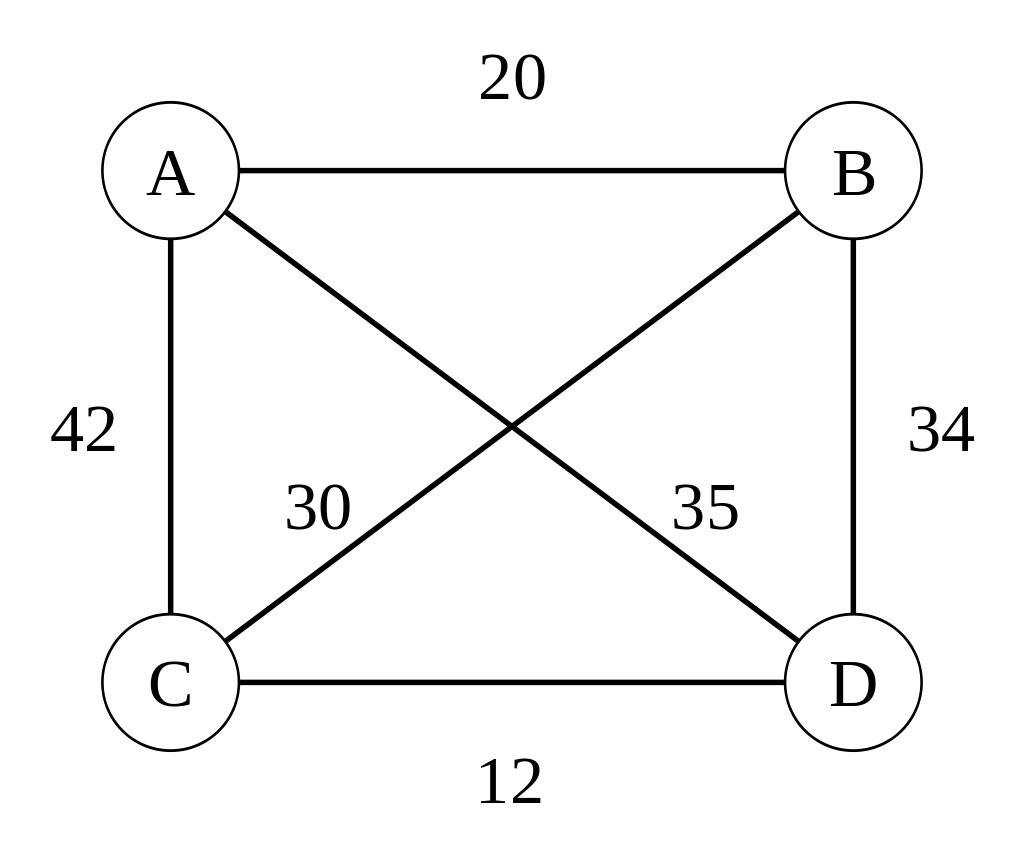
\includegraphics[scale=0.11]{files/SimmetricTSP.png}
        \caption{TSP simmetrico con 4 città}
    \end{figure}
\end{frame}

\begin{frame}{TSP simmetrico}
    Presenteremo un approccio risolutivo basato sul \textbf{Branch \& Bound}, che garantisce di trovare l'ottimo del problema in un tempo che può essere esponenziale. L'idea alla base di questa tecnica algoritmica è quella di partizionare con la fase di \textbf{Branching} lo spazio delle soluzioni in più sottospazi (non per forza disgiunti) la cui unione restituisca però tassativamente la regione iniziale. Avendo a che fare con spazi ridotti questi risulteranno di più facile analisi attraverso l'applicazione della fase di \textbf{Bounding}.
\end{frame}

\section{Formulazione matematica del TSP}
\begin{frame}{Formulazione matematica del TSP}
    Un circuito è detto hamiltoniano se su ogni nodo incidono esattamente due archi e, rimuovendo un nodo $n$ qualsiasi e i suoi due archi incidenti, si ottiene un albero sui rimanenti nodi $|V| - 2$. Una possibile formalizzazione matematica del TSP che tiene conto di questo risulta quindi la seguente:
    \begin{equation*}
      \begin{split}
        \min z = & \sum_{(i,j) \in E} c_{ij} \cdot x_{ij}\\
        (1)\:\:\:\:\:\: & \sum_{j \in V, i \neq j} x_{ij} = 2 \:\:\:\:\:\: \forall i \in V \\
        (2) \:\:\:\:\:\: & \sum_{(i,j)\in E, i, j \neq n} x_{ij} = |V|-2 \\
        (3) \:\:\:\:\:\: & \sum_{(i,j) \in E(U)} x_{ij} \leq |U| - 1 \:\:\:\:\:\: \forall\: U \subseteq V\setminus\{n\} : |U| \geq 3 \\
        (4) \:\:\:\:\:\: & x_{ij} \in \{0,1\} \:\:\:\:\:\: \forall (i,j) \in E\\
      \end{split}
    \end{equation*}
\end{frame}

\begin{frame}{Formulazione matematica del TSP - Dettagli}
    In dettaglio, il vincolo (1)
    \begin{equation*}
        \sum_{j \in V, i \neq j} x_{ij} = 2 \:\:\:\:\:\: \forall i \in V
    \end{equation*} impone che su ogni nodo $i \in V$ incidano esattamente due nodi.\newline
    
    I vincoli (2) e (3) invece
    \begin{equation*}
      \begin{split}
        (2) & \:\:\:\:\:\:  \sum_{(i,j)\in E, i, j \neq n} x_{ij} = |V|-2 \\
        (3) & \:\:\:\:\:\:  \sum_{(i,j) \in E(U)} x_{ij} \leq |U| - 1 \:\:\:\:\:\: \forall\: U \subseteq V\setminus\{n\} : |U| \geq 3\\
      \end{split}
    \end{equation*}
    garantiscono che una volta scelto un nodo $n$, $V \setminus \{n\}$ risulti un albero e quindi abbia $|V|-2$ archi e sia privo di circuiti.
\end{frame}

\begin{frame}{Formulazione matematica del TSP - Dettagli}
    \begin{equation*}
      \begin{split}
        (3) \:\:\:\:\:\: & \sum_{(i,j) \in E(U)} x_{ij} \leq |U| - 1 \:\:\:\:\:\: \forall\: U \subseteq V\setminus\{n\} : |U| \geq 3
      \end{split}
    \end{equation*}
    Dato un sottoinsieme di nodi $U \subseteq V$ definiamo $E(U)$ come l'insieme di archi $\{ (i,j) \:|\: i,j \in U \}$. Osservando che ogni circuito sui nodi in $U$ deve avere $|U|$ archi in $E(U)$, per eliminare i circuiti abbiamo inserito il vincolo (3). Imponiamo $|U| \geq 3$, poiché se fosse per esempio uguale a 2 allora $E(U)$ conterrebbe solamente l'arco tra i due nodi e non ci sarebbe alcun circuito.
    
    Il vincolo (4) infine
    \begin{equation*}
      \begin{split}
        (4) \:\:\:\:\:\: & x_{ij} \in \{0,1\} \:\:\:\:\:\: \forall (i,j) \in E\\
      \end{split}
    \end{equation*}
    modella il dominio delle variabili decisionali che assumono valore 1 se il corrispondente arco viene inserito nel circuito hamiltoniano e 0 altrimenti.
\end{frame}

\begin{frame}{Formulazione matematica del TSP - Idea di rilassamento}
    L'approccio che abbiamo scelto prevede un rilassamento Lagrangiano sul vincolo (1).\newline
    In questo modo il problema da risolvere risultante richiede di individuare il minimo 1-tree, una volta impostati i moltiplicatori lagrangiani $\lambda_i$ a 0, ossia eliminando il vincolo (1) per tutti i nodi tranne che per il nodo selezionato $n$.
\end{frame}

\section{Rilassamento Lagrangiano}
\begin{frame}{Rilassamento Lagrangiano}
    Una volta introdotti per ogni nodo dei moltiplicatori lagrangiani $\lambda_i$ e portando in funzione obiettivo il vincolo otteniamo:
    \begin{equation*}
        \begin{split}
             \min z = & \sum_{(i,j) \in E} c_{ij} \cdot x_{ij} + \sum_{k\in V} \lambda_k (2 - \sum_{j\in V, k\neq j} x_{kj})\\
            (5)\:\:\:\:\:\: & \sum_{j \in V, j \neq n} x_{nj} = 2 \\
            (2) \:\:\:\:\:\: & \sum_{(i,j)\in E, i, j \neq n} x_{ij} = |V|-2 \\
            (3) \:\:\:\:\:\: & \sum_{(i,j) \in E(U)} x_{ij} \leq |U| - 1 \:\:\:\:\:\: \forall\: U \subseteq V\setminus\{n\} : |U| \geq 3 \\
            (4) \:\:\:\:\:\: & x_{ij} \in \{0,1\} \:\:\:\:\:\: \forall (i,j) \in E\\
        \end{split}
    \end{equation*}
\end{frame}

\begin{frame}{Rilassamento Lagrangiano}
    Dato che abbiamo rilassato vincoli di uguaglianza si potranno considerare i migliori moltiplicatori lagrangiani non solo maggiori o uguali a 0, ma anche negativi. Per valori fissati dei vari $\lambda_k$ il rilassamento lagrangiano è facilmente risolvibile con una procedura (mostrata a breve) che consente di individuare l'1-tree di costo minimo.
    \newline
    \newline
    Riscrivendo la funzione obiettivo otteniamo:
    \begin{equation*}
         \min \sum_{(i,j)\in E} ( c_{ij} - \lambda_i - \lambda_j) \cdot x_{ij} + 2 \cdot \sum_{k \in V} \lambda_k
    \end{equation*}
    I costi associati agli archi risultano quindi aggiornati secondo:
    \begin{equation*}
        c_{ij}' = c_{ij} - \lambda_i - \lambda_j
    \end{equation*}
    Questo dà luogo ad un possible approccio risolutivo basato sul duale lagrangiano, che prevede di partire da una combinazione ammissibile di moltiplicatori come $\lambda_k = 0\:\: \forall k$, successivamente migliorando la soluzione provando nuovi moltiplicatori.
\end{frame}

\section{1-Tree}
\begin{frame}{1-Tree}
    Dato un grafo $G=(V,E)$ non orientato ed un suo nodo $n$ chiamiamo \textbf{1-tree} un sottografo $H = (V, E_H)$ di $G$ con $E_H \subset E$ e con le seguenti proprietà:
    \begin{enumerate}
        \item in $E_H$ sono presenti esattamente 2 archi incidenti sul nodo $n$;
        \item se escludiamo da $H$ il nodo $n$ (ed i suoi 2 archi incidenti su di esso) ne risulta un albero sull'insieme di nodi $V \setminus \{n\}$. \newline Alternativamente si può affermare che $H$ contiene un circuito passante per il nodo selezionato $n$.
    \end{enumerate}
    Da questa definizione segue che $|E_H| = |V|$.
\end{frame}

\begin{frame}{1-Tree}
    L'aspetto importante degli 1-tree è che ogni circuito hamiltoniano risulta un 1-tree, non è invece vero il viceversa. Se indichiamo con $S'$ l'insieme di tutti gli 1-tree calcolabili dato un grafo $G$ e con $S$ la regione ammissibile del TSP, abbiamo che $S \subset S'$.
    
    \begin{figure}
        \centering
         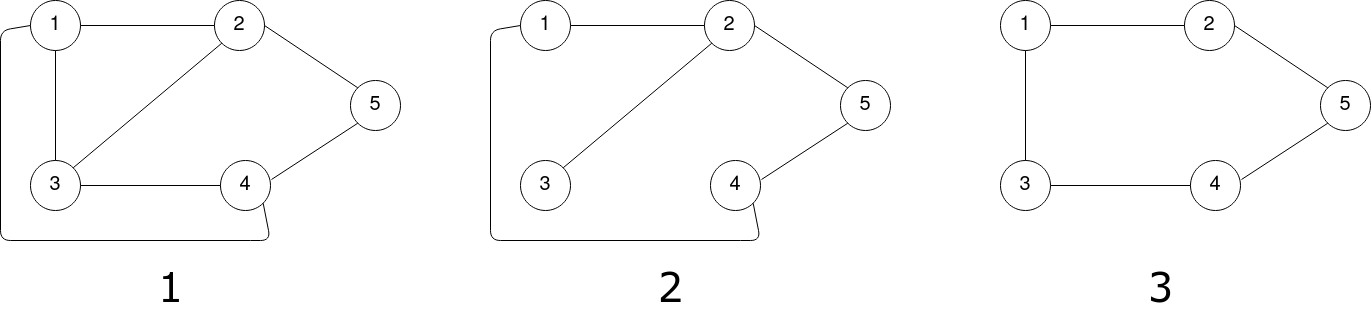
\includegraphics[scale=0.21]{files/1TreeEsempi.png}
        \caption{Nell'immagine 1 è proposta un'istanza di grafo $G(V,E)$ non orientato. I grafi 2 e 3 rappresentano due suoi 1-tree di cui 3 è anche un circuito hamiltoniano.}
    \end{figure}
       
   
\end{frame}

\begin{frame}{1-Tree}
    La formulazione matematica dell'1-tree risulta essere la seguente:
\begin{equation*}
    \begin{split}
        \min z = & \sum_{(i,j) \in E} c_{ij} \cdot x_{ij}\\
        (5)\:\:\:\:\:\: & \sum_{j \in V, j \neq n} x_{nj} = 2 \\
        (2) \:\:\:\:\:\: & \sum_{(i,j)\in E, i, j \neq n} x_{ij} = |V|-2 \\
        (3) \:\:\:\:\:\: & \sum_{(i,j) \in E(U)} x_{ij} \leq |U| - 1 \:\:\:\:\:\: \forall\: U \subseteq V\setminus\{n\} : |U| \geq 3 \\
        (4) \:\:\:\:\:\: & x_{ij} \in \{0,1\} \:\:\:\:\:\: \forall (i,j) \in E\\
    \end{split}
\end{equation*}
Come si può notare questa è identica al rilassamento lagrangiano precedentemente mostrato, una volta impostati i vari $\lambda_i = 0$.
\end{frame}

\begin{frame}{1-Tree}
    Una semplice procedura per calcolare un 1-tree di costo minimo e generare quindi un \textbf{lower bound} al problema del TSP segue i successivi passi:
    \begin{enumerate}[<+->]
        \item Si calcoli l'MST $T$ sul grafo ottenuto da $G$ scartando il nodo prescelto $n$ e tutti gli archi incidenti su di esso. Sia $E_T$ l'insieme degli archi della soluzione trovata;
        \item Si aggiungano ad $E_T$ i due archi $(n,k)$ e $(n,h)$ a distanza minima tra quelli incidenti sul nodo $n$.
        \item Si restituisca l'1-tree $H = (V, E_H)$ con $E_H = E_T \cup \{(n,k),(n,h)\}$.
    \end{enumerate}
\end{frame}

\begin{frame}{1-Tree}
    Il costo della procedura appena proposta risulta dominato dal calcolo dell'MST, risolvibile facilmente con un algoritmo greedy come quello di  Kruskal in tempo $O(m\cdot log\: n)$. La selezione al passo 2 della coppia degli archi di costo minore è ottenibile invece con una semplice scansione degli archi $O(m)$.
    \newline
    \newline
    Per quanto riguarda il calcolo e l'aggiornamento dell'\textbf{upper bound}, una volta calcolato un 1-tree se questo risulta anche un circuito hamiltoniano (ossia ogni nodo presenta grado 2) si può aggiornare l'upper bound se presenta un costo minore di quello per ora trovato. All'inizio del procedimento l'upper bound sarà impostato a $ + \infty$. 
\end{frame}

\section{Schema di Branch}
\begin{frame}{Schema di Branch}
    Ci occuperemo ora di mostrare come sarà partizionata la regione ammissibile $S$ in più sottoinsiemi.
    
    Se non stiamo analizzando il caso fortunato in cui \textit{la soluzione del rilassamento è un circuito hamiltoniano}, tale soluzione sarà allora un 1-tree che contiene esattamente un \textit{sottocircuito}. Dobbiamo introdurre una regola di suddivisione il cui scopo è impedire il formarsi nei nodi figli di tale sottocircuito.
\end{frame}

\begin{frame}{Schema di Branch}
    Indichiamo con $\{(i_1, j_1), (i_2,j_2),...,(i_r,j_r)\}$ gli archi che compongo tale sottocircuito.
    \newline
    \newline
    Schema di Branch:
    \begin{enumerate}[<+->]
        \item  Il primo nodo figlio verrà generato imponendo che l'arco $(i_1,j_1)$ non faccia parte della soluzione, ossia impostando $x_{i_{1}j_{1}} = 0$;
        \item Il secondo nodo figlio sarà ottenuto imponendo che sia presente l'arco $(i_1,j_1)$, ma sia assente l'arco $(i_2,j_2)$, ovvero impostando $x_{i_{1}j_{1}} = 1$ e $x_{i_{2}j_{2}} = 0$;
        \item Il procedimento continua in questo modo fino all' r-esimo figlio che avrà tutti i primi $r-1$ archi del sottocircuito e non conterrà l'ultimo, quindi $\forall k = 1,2,...,r-1 \:\:x_{i_{k}j_{k}} = 1$ e $x_{i_{r}j_{r}} = 0$.
    \end{enumerate}
     
\end{frame}

\begin{frame}{Schema di Branch}
    Ad ogni nodo saranno quindi associati due insiemi: 
    \begin{enumerate}
        \item $E_0$ contente tutti gli archi che non devono essere considerati;
        \item $E_1$ contenente tutti gli archi che devono essere in soluzione.
    \end{enumerate}
    Per ogni figlio si dovrà quindi risolvere un sottoproblema del tipo $S(E_0, E_1)$ contenente tutti i circuiti hamiltoniani formati sicuramente dagli archi in $E_1$ e privi degli archi in $E_0$.
    \newline
    \newline
    Per il calcolo del lower bound di un sotto problema $S(E_0, E_1)$ si usa la stessa procedura analizzata precedentemente imponendo però la presenza degli archi $E_1$ ed escludendo quelli in $E_0$ per il calcolo dell'MST e nella scelta dei 2 archi per il nodo $n$.
\end{frame}

\begin{frame}{Schema di Branch - 1}
    In particolare si risolverà sempre l'MST con Kruskal, ma inizializzando l'insieme $E_T$ con gli archi in $E_1$ non incidenti sul nodo $n$, invece che impostarlo come insieme vuoto.\newline
    Una volta fatto ciò, durante l'esecuzione dell'algoritmo non dovranno essere presi in considerazione gli archi in $E_0$.
    
    Ottenuto l'albero di copertura $T$, verranno aggiunti gli  archi incidenti in $n$ meno costosi.\newline
    Nel caso in cui $E_1$ dovesse contenere tali archi, essi saranno selezionati. In caso contrario si sceglieranno i migliori non presenti in $E_0$. 
\end{frame}

\begin{frame}{Schema di Branch - 2}
    Per il branching di un nodo interno, al sottocircuito individuato $\{(i_1, j_1), (i_2,j_2),...,(i_r,j_r)\}$ andranno tolti gli archi nell'insieme $E_1$ associato al nodo stesso, che non possono non essere presenti nei figli che saranno generati.\newline
    Una volta scremato l'insieme di archi si procederà nella stessa maniera e verranno estesi gli insiemi $E_0$ ed $E_1$ del padre per generare i vari figli necessari per proseguire la ricerca.
\end{frame}

\section{Chiusura dei nodi}
\begin{frame}{Chiusura dei nodi}
    Un nodo dell'albero di branch $P_i$ viene chiuso quando:
    \begin{enumerate}[<+->]
        \item $\hat{z} \leq LB(P_i)$, ossia quando il lower bound fornito è maggiore del migliore circuito hamiltoniano per ora trovato, in tal caso il nodo viene \textbf{chiuso per bound};
        \item non si riesce a calcolare un 1-tree per il nodo: in questo caso non esiste soluzione ammissibile per il rilassamento e il nodo sarà \textbf{chiuso per inammissibilità};
        \item l'1-tree generato dal rilassamento risulta essere un circuito hamiltoniano: il nodo verrà allora \textbf{chiuso perchè possibile candidato ottimo}.
    \end{enumerate}
    
\end{frame}

\begin{frame}{Chiusura dei nodi}
    Nell'ultimo caso delineato qualora il nodo presentasse anche un costo migliore e quindi minore dell'attuale soluzione trovata, questa verrebbe aggiornata.
    \newline
    \newline
    Se alcuni nodi risultano aperti la scelta del prossimo nodo su cui fare Branch ricade su quello che presenta il Lower Bound minore non ancora visitato.\newline
    Il nodo scelto in altri termini è quello che ci permette, in caso di ottimalità, di chiudere prima eventuali nodi aperti e terminare l'esecuzione. Un tale approccio viene detto \textbf{Best First}.
\end{frame}

\section{Analisi dell'implementazione}
\begin{frame}{Analisi dell'implementazione}
    L'intero codice implementativo può essere visionato direttamente presso la pagina \href{https://github.com/LorenzoSciandra/TesinaOttimizzazioneCombinatoria}{GitHub} della tesina. Seguirà in queste ultime slides un'analisi delle scelte rilevanti compiute e uno sguardo sull'esecuzione degli algoritmi discussi su istanze medio/grandi di grafi.
\end{frame}

\begin{frame}{Analisi dell'implementazione}
    Per quanto riguarda la struttura dati utilizzata abbiamo implementato il grafo e quindi anche l'1-tree che di volta in volta calcoliamo con delle \textbf{liste di adiacenze} realizzate con HashMap.\newline
    Nello specifico il grafo è visto come un'insieme di nodi, che a loro volta contengono insiemi di archi.
    
    Questa scelta risulta la più conveniente dal punto di vista della complessità per i compiti che dobbiamo svolgere. Un'esplorazione completa del grafo, così come lo spazio necessario per la memorizzazione richiede complessità $O(n+m)$, mentre la scansione degli adiacenti di un nodo risulta di costo minimo $O(|A(u)|)$, dove $A(u) = \{v \:|\: (u,v) \in E\}$.
\end{frame}

\begin{frame}{Analisi dell'implementazione}
    Tra le procedure più spesso eseguite troviamo sicuramente il calcolo del \textbf{Minimum Spanning Tree}, che viene ripetuto per ogni nodo dell'albero di Branch che andiamo a generare. Per tale calcolo abbiamo implementato l'algoritmo greedy proposto da Kruskal che presenta complessità ottima $O(m\cdot log\:n)$.
    
    Tale costo risiede principalmente nell'ordinamento decrescente iniziale degli archi, e nell'uso di Merge Find Set per controllare che un i-esimo arco possa essere incluso in soluzione con la certezza che non formi un ciclo.
\end{frame}

\begin{frame}{Analisi dell'implementazione}
    Per quanto riguarda l'individuazione del sottociclo all'interno di un 1-tree che non è un circuito hamiltoniano abbiamo usato una \textbf{Depht First search}, con complessità $O(n+m)$.
    
    L'idea è usare un vettore di padri per evitare di visitare più volte i nodi del grafo e per tener traccia del padre di ogni nodo. 
    
    Conclusa l'esplorazione in profondità del grafo, semplicemente partendo dal nodo candidato $n$ e procedendo con i vettori dei padri a ritroso, si individua il ciclo che ci servirà per il fare il Branch di un problema $P_i$.
\end{frame}

\begin{frame}{Analisi dell'implementazione}
    La procedura centrale per la risoluzione del TSP è firmata {\fontfamily{bch}\selectfont solveProblem()} e restituisce un'istanza della classe {\fontfamily{bch}\selectfont TSPResult}, contenente il ciclo hamiltoniano con costo minore e una serie di statistiche riguardo ai nodi analizzati nell'albero di Branch.
    \newline
    \newline
    Nel caso in cui non vi fosse un ciclo hamiltoniano nel grafo di partenza, viene restituito il grafo originale.
\end{frame}

\begin{frame}{Analisi dell'implementazione}
    Il metodo {\fontfamily{bch}\selectfont solveProblem()} richiama gli algoritmi precedentemente descritti assieme a molte altre procedure di supporto, al fine di gestire una {\fontfamily{bch}\selectfont PriorityQueue} di {\fontfamily{bch}\selectfont SubProblem} e terminando l'esecuzione non appena quest'ultima viene completamente svuotata in seguito alla chiusura di tutti i nodi per una delle ragioni precedentemente indicate. 
    \newline
    \newline
    \'E qui che risiede tutta la complessità della risoluzione del TSP simmetrico: questo metodo infatti richiama sottoprocedure polinomiali in tempo, ma il numero di {\fontfamily{bch}\selectfont SubProblem} che deve gestire può essere esponenziale.
\end{frame}

\begin{frame}{Analisi dell'implementazione}
    La gestione dell'insieme dei {\fontfamily{bch}\selectfont SubProblem} ancora aperti è stata realizzata con una coda di priorità \textbf{min-heap}, ossia con una struttura dati che presenta complessità $O(1)$ per leggere l'elemento con lower bound minore e $O(log\:n)$ per estrarre ed aggiungere un elemento.
\end{frame}

\begin{frame}{Analisi dell'implementazione}
    Terminiamo la relazione con l'analisi delle prestazioni della nostra implementazione.
    
    Su grafi banali come quello che verrà mostrato nell'esempio conclusivo della tesina il codice termina in qualche decina di millisecondi generando una manciata di nodi nell'albero di branch. Come abbiamo potuto toccare con mano, durante i nostri test, il tempo necessario per l'esecuzione dipende fortemente dal numero di archi che popolano il grafo. Esecuzioni su grafi sparsi di 100 nodi richiedono decine di secondi, mentre esecuzioni su grafi completi anche solo di 20 nodi richiedono manciate di minuti.
\end{frame}

\begin{frame}{Analisi dell'implementazione}
    Per ottenere un'analisi significativa delle prestazioni, abbiamo creato una classe Java {\fontfamily{bch}\selectfont BasicCompleteGraphGenerator} che ci permette di generare grafi completi una volta specificato il numero di nodi e il range entro il quale devono risiedere i costi degli archi. Ricordiamo che un grafo completo $G$ con $n$ nodi avrà $\frac{n\cdot (n-1)}{2}$ archi non orientati.
    
    
    Per dare maggiore rilevanza ai test effettuati abbiamo anche dato la possibilità di parallelizzare i calcoli su più thread. Una volta infatti che si è fatto il branch di un nodo e si ha generato tutti i figli di uno stesso livello questi possono tranquillamente essere computati simultaneamente per poi decidere se vadano chiusi per un qualche motivo o espansi con una ulteriore operazione di branch.
\end{frame}

\begin{frame}{Analisi dell'implementazione}
Mostriamo ora i dati che abbiamo raccolto con un calcolatore con processore AMD Ryzen 7 4.6GHz e 32 GB di RAM DDR4:
    \begin{center}
    \resizebox{6.5cm}{!}{
 \begin{tabular}{||c c c c c||} 
 \hline
 Thread & Nodi & Archi & Nodi generati & Tempo d'esecuzione\\ [0.5ex] 
 \hline\hline
 1 & 5 & 10 & 5 & 93ms\\ 
 \hline
 1 & 10 & 45 & 559 & 149ms\\
 %\hline
 %1 & 13 & 78 & 7293 & 250ms\\
 \hline
 1 & 15 & 105 & ... & ...\\
 \hline
 1 & 16 & 120 & ... & ...\\
 \hline
 1 & 17 & 136 & ... & ...\\
 \hline
 1 & 18 & 153 & ... & ...\\
 \hline
 \hline
 4 & 5 & 10 & 5 & 97ms\\ 
 \hline
 4 & 10 & 45 & 559 & 133ms\\
 \hline
 %4 & 13 & 78 & 7293 & 234ms\\
 %\hline
 4 & 15 & 105 & ... & ...\\
 \hline
 4 & 16 & 120 & ... & ...\\
 \hline
 4 & 17 & 136 & ... & ...\\
 \hline
 4 & 18 & 153 & ... & ...\\
 \hline
 \hline
 8 & 5 & 10 & 5 & 101ms\\ 
 \hline
 8 & 10 & 45 & 559 & 155ms\\
 %\hline
 %8 & 13 & 78 & 7293 & 223ms\\
 \hline
 8 & 15 & 105 & ... & ...\\
 \hline
 8 & 16 & 120 & ... & ...\\
 \hline
 8 & 17 & 136 & ... & ...\\
 \hline
 4 & 18 & 153 & ... & ...\\
 \hline
\end{tabular}
}
\end{center}


\end{frame}

\begin{frame}{Analisi dell'implementazione}
    I puntini nella tabella rappresentano esecuzioni che non sono terminate a causa della mancanza di RAM. Il {\fontfamily{bch}\selectfont Garbage Collector} di Java permette di eliminare tutte le classi non più utili, ma il numero di {\fontfamily{bch}\selectfont SubPorblem} che sono ancora attivi nella frontiera dell'albero di branch può essere esponenzialmente grande. Basti pensare al fatto che non tutti i {\fontfamily{bch}\selectfont SubProblem} rimangono aperti e generano figli, ma coloro che lo fanno possono avere un branching factor molto grande.
    
    
    Ovviamente tutto questo non ci sorprende più di tanto poichè rispecchia quella che è una procedura di risoluzione esponenziale per un problema NP-hard come il TSP.
\end{frame}

\end{document}
